\cotefile{123}
\scanpage{22}
\handwritten{\unsure{Massy} 22. 10. 1969}\\

Dear Kostant,\\

I read again through your papers in the \unsure{Maer.|Amer.} Journ. on \handwritten{``}\deleted{t}\handwritten{T}he principal three-dimensional subgroup ...\handwritten{''} and \handwritten{``}Lie group representations on polynom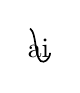
\begin{tikzpicture}[baseline=(letters.base),x=1em,y=1em]
\node[inner sep=0pt] (letters) at (0,0) {ai};
\handwritten{\draw[line width=.6pt] (-.30,.72) .. controls (-.04,.55) and (-.16,-.55) .. (.19,-.48) .. controls (.34,-.46) and (.44,-.22) .. (.42,-.16);}
\end{tikzpicture}l rings\handwritten{''}, prompted by some nice work of Brieskorn on Klein singularities. I very much appreciate this work of yours, and would appreciate getting reprints of any later work you may have available. As I already felt when your work appea\deleted{\unsure{k|r}}\handwritten{r}ed, it cries for careful reconsideration in the framework of \deleted{\unsure{a|A}}\handwritten{A}lg. Geometry, and suggests number of interesting problems. I wonder if you know the answer to some of them. For instance, I feel it would be of interest to classify (for a given complex simple adjoint Lie group, say) quadr\deleted{\unsure{a|u}}uples $(\mathrm{T},\mathrm{B},\mathrm{T}',\mathrm{B}')$, where $\mathrm{T}$ and $\mathrm{T}'$ are maximal tori ``in apposition\handwritten{''} (in your terminology), and $\mathrm{B}$ and $\mathrm{B}'$ Borel subgroups of $\mathrm{G}$ containing $\mathrm{T}$ resp. $\mathrm{T}'$. The number of conjugacy classes of such animals is equal to $\operatorname{card}(\mathrm{W})^{2}/\mathrm{hz}\handwritten{\phi}(\mathrm{h})$, where $\deleted{\unsure{\mathrm{H}|\mathrm{W}}}\handwritten{W}$ is the Weyl group, $\mathrm{h}$ the Coxeter number, $\mathrm{z}$ the order of the center\inserted{\handwritten{of $\widetilde{G}$}}, and $\handwritten{\phi}(\mathrm{h})=\operatorname{card}(\underline{\mathrm{Z}}/\mathrm{h}\underline{\mathrm{Z}})^{\handwritten{*}}$ is the Euler indicatrix; if you want to classify such data with moreover a\deleted{n} \inserted{generating} element (principal regular in your terminology) given for the finite group of order $\mathrm{h}$ $\mathrm{T}\handwritten{\cap}\mathrm{N}(\mathrm{T}')$, then we get $\operatorname{card}(\mathrm{W})^{\handwritten{2}}/\mathrm{hz}$ choices. One of the reasons I think this question is interesting is that the stability subgroup in $\mathrm{G}$ of such a quadruple is $\mathrm{T}\handwritten{\cap}\mathrm{T}'=\mathrm{e}$,\handwritten{\textsuperscript{*}} hence such a structure makes $\mathrm{G}$ entirely ``rigid'' up to exterior automorphisms. Among the first questions one may wish to ask in this direction are the following: is it true that for some, or for all, such quadruples, $\mathrm{B}$ and $\mathrm{B}'$ are ``in general position'' i.e. $\mathrm{B}\handwritten{\cap}\mathrm{B}'$ is a torus (necessarily maximal), so that $\mathrm{B}$ and $\mathrm{B}'$ are ``opposite'' to each other with respect to the latter ? Is there in any sense a \uline{distinguished} conjugacy class of such quadruples (which should then be, of course, invariant by action of exterior automorphisms) ? What are the groups of automorph\deleted{\unsure{k|i}}isms of such quadr\deleted{a}uples (they

\margin{\handwritten{* NB: $N(T)\cap N(T')$ is an extension of $(\mathbb{Z}/h\mathbb{Z})^{*}$ by $\mathbb{Z}/h\mathbb{Z}\times \underset{\substack{\tikz[scale=.2]{\draw (0,0)--(.2,.6);}
\\\text{center of }\widetilde{G}}}{Z}\deleted{\unsure{(G)|(\widetilde{G})}}$, hence of order $hz\varphi(h)$}}
% The short oblique leader and its lower annotation are retained below Z.
% The handwritten transposition stroke crosses the original typed ``ai'' in ``polynomail''; no replacement letters have been supplied.
% archive sheet number: 21

\scanpage{23}
are isomorphic to subgroups of the group of exterior automorphisms of $\mathrm{G}$) ?

In a different direction, it would be\handwritten{\raisebox{.6ex}{$\vert$}}interesting to know more about the canonical morphism $\underline{\mathrm{g}}\handwritten{\longrightarrow}\underline{\mathrm{h}}/\mathrm{W}$, where $\underline{\mathrm{g}}$ is the Lie algebra of $\mathrm{G}$ and $\underline{\mathrm{h}}$ a Cartan subalgebra, and of the orbits of $\mathrm{G}$ on $\underline{\mathrm{g}}$, and the analogous morphism of Steinberg $\mathrm{G}\handwritten{\longrightarrow}\mathrm{T}/\mathrm{W}$ and the orbits of $\mathrm{G}$ acting on itself. Do you know for instance exactly how varies the rank (= rang of the tangent map) of this \deleted{\unsure{applicati}} map ? There are some reasons to believe that \deleted{this} for points of unipotent orbits of dimension $\inserted{\handwritten{n-}}\mathrm{r}-2$ (just \deleted{the next lower after}\inserted{the next lower after} the maximal dimension $\mathrm{n}-\mathrm{r}$), the rank is $\mathrm{r}-1$ in case all roots have same length (that is the corresponding diagrams $\mathrm{A}_{\deleted{\unsure{\mathrm{n}|\mathrm{r}}}\mathrm{r}},\mathrm{D}_{\deleted{\mathrm{n}}\mathrm{r}},\mathrm{E}_{\handwritten{6}},\mathrm{E}_{\handwritten{7}},\mathrm{E}_{\handwritten{8}}$ are those corresponding to Klein singularities), and $\handwritten{<}\mathrm{r}-1$ in \inserted{\handwritten{all}} other cases; in the first case, I would expect that there is just one orbit as stated, by the way, and maybe this property will be characteristic of the ``homogene\deleted{\unsure{a|u}}ous'' case when all roots have same length. Also, what can be said of the dim\deleted{\unsure{o|e}}ension of the set of all Borel subgroups containing a given element $\mathrm{g}\handwritten{\in}\mathrm{G}$, resp. whose Lie algebra contains a given element $\mathrm{x}\handwritten{\in}\underline{\mathrm{g}}$ ? If $2\mathrm{N}=\mathrm{n}-\mathrm{r}$ is the number of roots and if the dimension of the orbit of the given element is $2\mathrm{N}-2\mathrm{i}$, I would expect the dimension of the previous variety to be equal to $\mathrm{i}$; the inequality $\handwritten{\leqslant}\mathrm{i}$ would imply, by generalizing a depth argument of Br\deleted{\unsure{e|i}}i\deleted{\unsure{i|e}}eskorn, that the singularities of the fibers of your map $\underline{\mathrm{g}}\handwritten{\longrightarrow}\underline{\mathrm{h}}/\mathrm{W}$ (resp. Steinberg's $\mathrm{G}\handwritten{\longrightarrow}\mathrm{T}/\mathrm{W}$ in case $\mathrm{G}$ is simply connected instead of adjoint) are ``rational'', i.e. i\deleted{s}f $\mathrm{F}$ is such a fiber and $\mathrm{F}'\overset{\mathrm{f}}{\handwritten{\longrightarrow}}\mathrm{F}$ a resolution of singularities of $\mathrm{F}$, t\deleted{e}h\deleted{h}en $\mathrm{R}^{\mathrm{i}}\mathrm{f}_{\handwritten{*}}(\underline{\mathrm{O}}_{\mathrm{F}'}^{\deleted{\unsure{\mathrm{t}|*}}})=0$ for $\mathrm{i}\handwritten{>}0$. Maybe the answer \deleted{\unsure{ot|to}}\handwritten{to} most of the questions I am asking are well known and I am just ignorant; for some of them, it would indeed be scandalous that the experts do not know the answer ! In any case, I would be grateful for any comment you would have on any of my questions.

Sincerely yours\\
\handwritten{A\,\unsure{Grothendieck}}\\
% The vertical pen stroke at ``beinteresting'' is retained as a raised bar; no silent space has been supplied.
% archive sheet number: 22

\scanpage{28}
\mspage{\handwritten{22}}
% archive sheet number: 27 (inverted at the upper right)
% A single long vertical cancellation stroke runs through the typescript, from the opening paragraph into the footnote. The three enclosing deletion macros preserve this page-wide cancellation; inner deletion macros preserve the local revisions.

\deleted{un morphisme de topos $\mathrm{u}:\mathrm{E}\handwritten{\longrightarrow}\mathrm{E}'$, et ce dernier sera ``unique à isomorphisme unique près'' en termes de la donnée $\mathrm{u}^{\handwritten{*}}$ resp. $\mathrm{u}_{\handwritten{*}}$, en un sens assez clair, et qui sera d'ailleurs entièrement explicité plus bas \handwritten{(\deleted{\unsure{2|3}}3.2.1)}}

\deleted{\deleted{\unsure{2|3}}\handwritten{3}.1.2. Si $\mathrm{u}:\mathrm{E}\handwritten{\longrightarrow}\mathrm{E}'$ est un morphisme de topos, il résulte des propriétés des foncteurs adjoints \inserted{\handwritten{(I 2.11)}} que le foncteur image directe $\mathrm{u}_{\handwritten{*}}:\mathrm{E}\handwritten{\longrightarrow}\mathrm{E}'$ commute aux limites projectives, et le foncteur $\mathrm{u}^{\handwritten{*}}:\mathrm{E}'\handwritten{\longrightarrow}\mathrm{E}$ commute aux limites inductives \deleted{\unsure{(2.11)|(2.1)|(I 2.11)}}\handwritten{(${}^{*}$)}.Comme on suppose de plus que ce dernier \inserted{\handwritten{est \unsure{exact} à gauche i.e.}} commute aux limites projectives finies, on voit donc en particulier que $\mathrm{u}^{\handwritten{*}}$ \uline{est} \deleted{exac} \uline{exact}. \inserted{On peut donc dire que} \uline{\deleted{C}\handwritten{c}'est \deleted{donc} le foncteur image inverse} $\mathrm{u}^{\handwritten{*}}$ \deleted{qui}, dans le couple $(\mathrm{u}_{\handwritten{*}},\mathrm{u}^{\handwritten{*}})$, \uline{qui possède les propriétés d'exactitude les plus remarquables}, \deleted{assurant} Ces propriétés assurent que pour toute espèce de structure algébrique \inserted{\handwritten{$\Sigma$}}\deleted{qui peut} dont les données peuvent se décrire en termes de données de flèches entre les ensembles de base et des ensembles déduits de ceux-ci par application répétée d'opérations de limites projectives finies et de limites inductives quelconques, \inserted{\handwritten{et pour}} tout \handwritten{``}objet de $\underline{\mathrm{E}}'$ muni d'une structure d'espèce $\handwritten{\Sigma}$'' (notion qui a un sens grâce aux propriétés d'exactitude \deleted{de} internes du topos $\mathbb{E}'$ (II 4.1)), son image \deleted{inverse} par $\mathrm{u}^{\handwritten{*}}$ est muni des mêmes structures. Plutôt que d'entrer dans la tâche peu engageante de donner un sens précis à cet énoncé et de le justifier de façon formelle, nous conseillons au lecteur de \inserted{l'expliciter et de} se convaincre de sa validité pour des espèces de structure telles que celle de groupe, d'anneau, de module sur un anneau, de comodule \deleted{ou de bimodule} sur un anneau, de bigèbre sur un anneau, de torseur sous un groupe. (Dans ces exemples, les trois premières espèces de structure se définis}
% The last word is cut at the right image edge after the visible fragment ``définis''; no unseen ending is supplied. The parenthesis is open on the source page.

\margin{\handwritten{\deleted{\unsure{(I 2.11)|(I 4.11)|(I 4.1)}}.}}

\handwritten{\figure{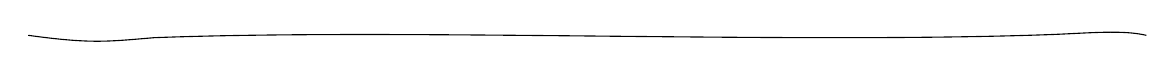
\begin{tikzpicture}[x=1cm,y=1cm]
\draw[line width=.4pt] (0,.03) .. controls (.8,-.08) and (1.0,-.05) .. (1.6,0) .. controls (4.8,.12) and (9.7,-.08) .. (13.0,.04) .. controls (13.5,.06) and (13.9,.10) .. (14.2,.03);
\end{tikzpicture}}}

\deleted{($\handwritten{*}$) \deleted{On peut} \deleted{d}\handwritten{D}'ailleurs \deleted{\unsure{vérifier que}}\inserted{\handwritten{(1.5 et 1.8)}}, pour un foncteur $\mathrm{u}_{\handwritten{*}}:\mathrm{E}\handwritten{\longrightarrow}\mathrm{E}'$ resp. $\mathrm{u}^{\handwritten{*}}:\mathrm{E}'\handwritten{\longrightarrow}\mathrm{E}$ donné, \deleted{d}\handwritten{c}e foncteur admet un adjoint à gauche (resp. à droite si et seulement si il commute aux \inserted{$\underline{\mathrm{U}}$-}limites projectives (resp. aux $\underline{\mathrm{U}}$-limites inductives). \deleted{\unsure{D'ailleurs}, c'est une conséquence immédiate de 1.2.\unsure{(ii)|(iii)|(i)}}}
% The right edge after ``droite'' is cropped; no unseen closing parenthesis has been added.

\scanpage{40}
\mspage{\handwritten{23}}
% archive sheet number: 39 (inverted, upper left)
% The two loop-and-stem signs below reproduce the handwritten linking marks; they are not read as letters.
% The top and bottom marginal continuations are placed at their marked insertion points.
sent en termes de limites projectives finies exclusivement, tandis que les autres notions impliquent implicitement des constructions faisant appel également à des limites inductives)\handwritten{)}.
\inserted{\handwritten{De plus, le foncteur $u^{*}$ ``\uline{commute}'' à toutes
\tikz[baseline=-0.3ex,scale=.18]{\draw (0,1.3)--(0,.15) .. controls (-.4,-.2) and (.4,-.2) .. (0,.15);}
\figure{\begin{tikzpicture}
\node[inner sep=6pt,text width=.88\linewidth,align=left] (n) {\tikz[baseline=-0.3ex,scale=.18]{\draw (0,1.3)--(0,.15) .. controls (-.4,-.2) and (.4,-.2) .. (0,.15);}les opérations fonctorielles \deleted{\illegible{1}} habituelles faites en termes de telles structures, plus précisément à toutes les opérations qui \inserted{peuvent} s'exprime\deleted{nt}\unsure{r} en termes de $\varinjlim$ et de $\varprojlim$ finies: constructions d'objets libres (groupes ou modules libres, p.ex.) engendrés par un objet, produits tensoriels (cf. \S 6 plus bas) etc.};
\draw ([yshift=2mm]n.north west) .. controls ([xshift=-2mm]n.west) and ([xshift=-1mm]n.south west) .. (n.south west) -- ([xshift=1mm]n.south) -- ([xshift=2mm,yshift=2mm]n.south) -- ([yshift=2mm]n.south east);
\end{tikzpicture}}}}

\margin{\handwritten{\figure{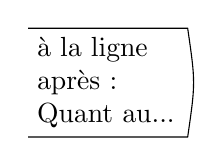
\begin{tikzpicture}\node[align=left,text width=1.8cm,inner sep=3pt] (n) {à la ligne après : Quant au...};\draw (n.north west)--(n.north east) .. controls ([xshift=1mm]n.east) .. (n.south east)--(n.south west);\end{tikzpicture}}}}
% The opposing pen brackets mark the paragraph break immediately before Quant au.
\handwritten{\tikz[baseline=-.6ex,scale=.18]{\draw (0,1.5)--(.5,1.4)--(.6,0)--(0,-.15);\draw (1.4,1.4)--(.9,1.35)--(.9,-.1)--(1.5,-.15);}}
Quant au foncteur image directe $\mathrm{u}_{\handwritten{*}}$\inserted{$:\mathrm{E}\handwritten{\longrightarrow}\mathrm{E}'$}, qui commute aux limites projectives, il ``respecte'' \inserted{par suite} toute structure algébrique sur un objet (ou une famille d'objets) de $\mathrm{E}$, définissable en termes de limites projectives \inserted{exclusivement} (telles les structures de groupe, d'anneau ou de module sur un anneau, \deleted{dans}\inserted{parmi} les exemples précédents). Par \deleted{f}contre, le foncteur $\mathrm{u}_{\handwritten{*}}$ n\deleted{e}'est en général pas exact à droite i.e. il ne commute pas en général aux limites inductives finies, et même ne transforme pas en général épimorphisme en épimorphisme\handwritten{\unsure{;|,}} (c'est d'ailleurs \deleted{\unsure{comme} nous le verrons au} ce défaut d'exactitude du foncteur $\mathrm{u}_{\handwritten{*}}$ qui est \handwritten{à} la source de ces propriétés cohomologiques, qui seront étudiées (du point de vue de l'algèbre homologique commutative) dans l'exposé suivant\handwritten{)}.
\inserted{\handwritten{Par suite, il ne \deleted{transforme pas}\inserted{s'étend pas}, en général,
\tikz[baseline=-.3ex,scale=.18]{\draw (0,0)--(.05,1.3) .. controls (-.35,1.65) and (.45,1.65) .. (.05,1.3);}
\figure{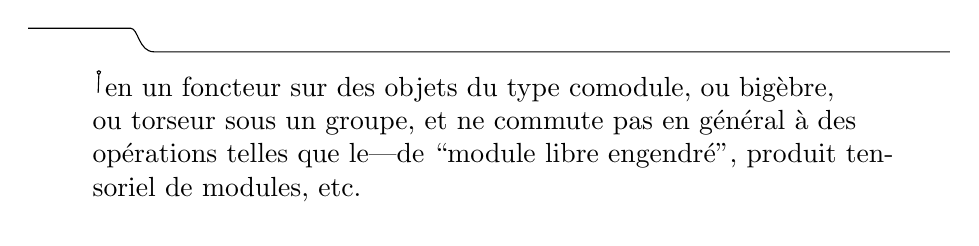
\begin{tikzpicture}
\node[inner sep=6pt,text width=.88\linewidth,align=left] (n) {\tikz[baseline=-.3ex,scale=.18]{\draw (0,0)--(.05,1.3) .. controls (-.35,1.65) and (.45,1.65) .. (.05,1.3);}en un foncteur sur des objets du type comodule, ou bigèbre, ou torseur sous un groupe, et ne commute pas en général à des opérations telles que \deleted{\unsure{le|de}} ``module libre engendré'', produit tensoriel de modules, etc.};
\draw ([xshift=-6mm,yshift=3mm]n.north west)--([xshift=7mm,yshift=3mm]n.north west) .. controls ([xshift=8mm,yshift=3mm]n.north west) and ([xshift=8mm]n.north west) .. ([xshift=10mm]n.north west)--(n.north east);
\end{tikzpicture}}}}

\deleted{2}\handwritten{3}.1.3. En pratique, lorsqu'on \deleted{se donne}\inserted{est \inserted{\handwritten{en}} présenced'}un foncteur $\mathrm{f}:\mathrm{E}\handwritten{\longrightarrow}\mathrm{F}$ d'un $\underline{\mathrm{U}}$-topos dans un autre, il y a lieu d'en expliciter \inserted{\handwritten{toutes}} les propri\deleted{t}é\deleted{é}tés d'exactitude, \deleted{y compris et de déterminer s'il admet un foncteur exact} y compris l'existence éventuelle de foncteurs adjoints à gauche ou à droite (cf. la note de bas de page précédente), pour parvenir à une compréhension de la ``nature géométrique'' de $\mathrm{f}$, \deleted{qui} compréhension qui sera généralement un guide indispensable pour \deleted{l'}\inserted{une}intuition géométrique correcte de la situation. Ainsi, s'il s'avère que $\mathrm{f}$ commute aux limites inductives quelconques et aux limites projectives finies, il y a lieu d'écrire $\mathrm{f}$ sous la forme
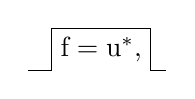
\begin{tikzpicture}[baseline=(n.base)]\node[inner sep=3pt] (n) {$\mathrm{f}=\mathrm{u}^{\handwritten{*}}$,};\handwritten{\draw ([xshift=-3mm]n.south west)--(n.south west)--(n.north west)--(n.north east)--(n.south east)--([xshift=2mm]n.south east);}\end{tikzpicture}
où
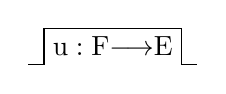
\begin{tikzpicture}[baseline=(n.base)]\node[inner sep=3pt] (n) {$\mathrm{u}:\mathrm{F}\handwritten{\longrightarrow}\mathrm{E}$};\handwritten{\draw ([xshift=-2mm]n.south west)--(n.south west)--(n.north west)--(n.north east)--(n.south east)--([xshift=2mm]n.south east);}\end{tikzpicture}
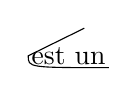
\begin{tikzpicture}[baseline=(n.base)]\node[inner sep=1pt] (n) {est un};\handwritten{\draw ([xshift=2mm,yshift=2mm]n.north)--(n.west) .. controls (n.south west) .. (n.south east);}\end{tikzpicture}
morphisme de topos, i.e. d'interpréter $\mathrm{f}$ comme un foncteur ``image inverse'' par une ````application continue'' de topos. Lorsque $\mathrm{f}$ commute aux limites projectives quelconques, donc qu'il admet un adjoint à gauche,\deleted{$\mathrm{g}$}
